\documentclass[11pt,a4paper,oneside]{article}
\usepackage{titling}
\newcommand{\subtitle}[1]{%
  \posttitle{%
    \par\end{center}
    \begin{center}\large#1\end{center}
    \vskip0.5em}%
}
\title{\textbf{Group 21: Cognitive Modeling - Lab 3}}
\date{\today}
\author{Olusanmi Hundogan - 6883273\\
Evangelia Giannikou - 6988229\\
}
% \pagenumbering{gobble}
\pagenumbering{arabic}

% \usepackage{eurosym}
\usepackage{hyperref}
% \usepackage{subfig}
\usepackage{amsmath}
\usepackage{amssymb}
\usepackage{tabularx,booktabs}
\usepackage{multicol}
\usepackage{array}
\usepackage{float}
\usepackage[english]{babel}
\usepackage{wrapfig}
\usepackage{graphicx}
\usepackage[font=scriptsize]{caption}
\usepackage{subcaption}


\setcounter{secnumdepth}{0}
\newcolumntype{M}[1]{>{\centering\arraybackslash}m{#1}}
\usepackage[backend=biber, sorting=none]{biblatex}
\usepackage[margin=1in]{geometry}
\addbibresource{references.bib}

\newcommand{\icol}[1]{% inline column vector
  \left(\begin{smallmatrix}#1\end{smallmatrix}\right)%
}

\newcommand{\irow}[1]{% inline row vector
  \begin{smallmatrix}(#1)\end{smallmatrix}%
}

\begin{document}

\maketitle

\section{Question 1}
\label{Q1}
\textit{Show two graphs: (i) what the probability of using threshold looks like on the scale 1-250 cm; (ii) the graph of the function $\sigma$ on the same scale. Second, state which degree point has the highest probability of being used as a threshold, and on which degree point it is most likely the speaker will use the adjective tall. If the two values differ or are the same, say in a few words why you think this is so.}\\

In Figure \ref{fig:q1_threshold}, the probability of using threshold on the scale 1-250 cm is shown. The highest degree point is when threshold $ \theta = 0.083$, and height = 184 cm.

\begin{figure}[H]
    \centering
    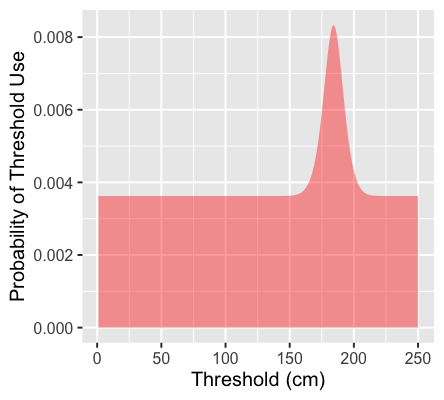
\includegraphics[width=\textwidth]{figs/Question_1_threshold.png}
    \caption{The graph shows the probability of using a threshold on a scale of 1-250 cm.}
  \label{fig:q1_threshold}
\end{figure}

Similarly, in Figure \ref{fig:q1_sigma}, it is shown the graph of the function $\sigma$ on the same scale. The function expresses the likelihood that the speaker will use the adjective 'tall' to tell how tall is something. In the graph, the highest degree point is 1 and height = 255 cm, which means that it is definite that the speaker will use the adjective tall when threshold $ \theta = 1$ and height = 255 cm. As the value decreases, the likelihood is diminishing as well. By using the probability of threshold $\theta = 0.083$ in Figure \ref{fig:q1_threshold}, the speaker is most likely to use the adjective 'tall' for heights greater than 184 cm.

\begin{figure}[H]
    \centering
    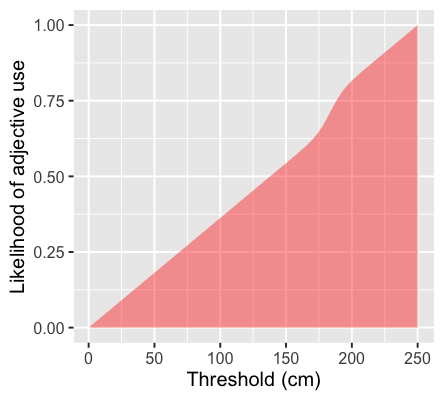
\includegraphics[width=\textwidth]{figs/Question_1_sigma.png}
    \caption{The graph shows the function $\sigma$ on a scale 1-250 cm.}
  \label{fig:q1_sigma}
\end{figure}



\section{Question 2}
\label{Q2}
\textit{}\\

\section{Question 3}
\label{Q3}
\textit{}\\

\section{Question 4}
\label{Q4}
\textit{}\\

\section{Question 5}
\label{Q5}
\textit{}\\

\section{Bonus question}
\label{bonus}
\textit{}\\

\clearpage 
\printbibliography
\end{document}